\documentclass[a4paper]{report}
\usepackage[utf8]{inputenc}
\usepackage[italian]{babel}
\usepackage{graphicx}
\usepackage{listings}
\graphicspath{ {./} }
\usepackage{color}
\definecolor{lightgray}{rgb}{.9,.9,.9}
\definecolor{darkgray}{rgb}{.4,.4,.4}
\definecolor{purple}{rgb}{0.65, 0.12, 0.82}

\lstdefinelanguage{JavaScript}{
  keywords={typeof, new, true, false, catch, function, return, null, catch, switch, var, if, in, while, do, else, case, break},
  keywordstyle=\color{blue}\bfseries,
  ndkeywords={class, export, boolean, throw, implements, import, this},
  ndkeywordstyle=\color{darkgray}\bfseries,
  identifierstyle=\color{black},
  sensitive=false,
  comment=[l]{//},
  morecomment=[s]{/*}{*/},
  commentstyle=\color{purple}\ttfamily,
  stringstyle=\color{red}\ttfamily,
  morestring=[b]',
  morestring=[b]"
}

\lstset{
   language=JavaScript,
   backgroundcolor=\color{lightgray},
   extendedchars=true,
   basicstyle=\footnotesize\ttfamily,
   showstringspaces=false,
   showspaces=false,
   numbers=left,
   numberstyle=\footnotesize,
   numbersep=9pt,
   tabsize=2,
   breaklines=true,
   showtabs=false,
   captionpos=b
}



\title{
    Affluencer \\
    \large Applicazioni e Servizi Web
}

\author{
    Daniele Gambaletta - 924643\{daniele.gambaletta@studio.unibo.it\}
    \\
    Michele Durante - 718472 \{michele.durante3@studio.unibo.it\}
    \\
    Giacomo Pasini - 885317 \{giacomo.pasini5@studio.unibo.it\}
}

\date{Luglio 2021}

\begin{document}

\maketitle

\pagebreak

\tableofcontents

\pagebreak

\chapter{Introduzione}

Il 9 Marzo 2020 è stato l'inizio del primo lockdown in Italia, causato dalla corrente pandemia di Coronavirus. Sin da allora sono state diverse le situazioni di paura e incertezza da parte degli imprenditori, soprattutto per coloro che non disponevano di un elevato budget economico. L'impreparazione del governo e l'indebolimento delle strutture sanitarie ha fatto sì che molte piccole attività chiudessero, rassegnate di fronte allo scarso supporto economico e alle difficoltà di aderire alle procedure sanitarie. Quest'ultima parte ha creato non poche diatribe tra gli imprenditori e il comitato tecnico scientifico: sebbene i locali venissero messi in sicurezza e controllati dalle forze dell’ordine, l'introduzione del coprifuoco serale e il take-away come unica opzione per i ristoratori hanno portato gli imprenditori a protestare e ad attivarsi autonomamente, non curanti delle multe e dei potenziali rischi di contagio.

Una delle imposizione che sono state applicate è la riduzione della capacità massima di persone presenti contemporaneamente in un locale. La categoria che è stata più colpita da questa norma è sicuramente quella dei ristoratori, poiché data la natura delle loro attività non permette, in un tempo limitato, di ottenere introiti come normalmente avverrebbe utilizzando la capacità massima dell'edificio (il servizio d'asporto ha consentito per alcuni di alleviare la situazione e di raggiungere il minimo sufficiente a mantenere in piedi l'attività). La maggior parte delle restanti attività hanno avuto sì un impatto sulle finanze, ma generalmente più ammortizzato. Tuttavia anche per loro è risultato problematico gestire gli ingressi, garantendo in contemporanea un ambiente sicuro per i clienti.

\pagebreak

\chapter{Requisiti}

Il progetto Affluencer si presenta come uno strumento in mano sia ai negozianti che ai privati cittadini.
%
Il portale sarà accessibile sia da desktop che da smartphone, adattando la vista al dispositivo utilizzato.
%
Per accedere è necessaria una connessione a Internet.

\section{Caratteristiche principali}

Tutti coloro che dispongono di un'attività possono registrarsi al portale come negozio ed ottenere un misuratore di flusso in grado di aggiornare in tempo reale l'affluenza nel proprio locale.
%
Ogni attività registrata ha la sua pagina personale modificabile, contenente le informazioni sull’attività e le misurazioni di flusso inviate dai sensori.
%
Un servizio di annunci aiuta a comunicare in modo veloce ai propri clienti.

I privati possono registrarsi con un account di tipo cliente e cercare i negozianti direttamente da una mappa oppure mediante barra di ricerca, con la possibilità di salvare i propri preferiti per una rapida consultazione.
%
È possibile scrivere recensioni sui negozi visitati e ricevere un feedback dai negozianti.
%
Inoltre, i clienti possono segnalare personalmente il numero di persone presenti nel locale e/o in coda all'ingresso.
%
Infine, un servizio di prenotazioni aiuta il negoziante a prevedere l'affluenza per coloro che intendono raggiungere il locale in un determinato orario.
%
Dal profilo cliente è possibile visualizzare e gestire negozi preferiti, prenotazioni e recensioni.
%
Grafici e dati presenti sulle pagine dei negozi aiutano privati e negozianti a conoscere gli orari di punta e a valutare il periodo adatto per effettuare gli acquisti.

\section{Features}

\textbf{Interactive Map}: Utilizzando il GPS, un utente può usare la mappa interattiva e ricevere le notifiche riguardo alla situazione dei suoi negozi preferiti, oppure inviare una segnalazione relativa all’affluenza in un negozio, in base alla sua posizione.
%

\textbf{Notifications}: Un sistema di notifiche manda ai clienti i reminder delle prenotazioni effettuate.
%

\textbf{IoT sensors}: L’applicazione gestisce i dati di centinaia di sensori IoT (simulati lato server), integrandoli ai dati relativi alle segnalazioni dei clienti e alle prenotazioni effettuate.
%

\textbf{Data visualization}: Nelle pagine dei negozi vengono visualizzati grafici che integrano i suddetti dati.

\chapter{Design}

Per lo sviluppo del progetto è stato adottato il metodo agile, garantendo ai componenti del team di operare in modo autonomo e iterativo.
%
In particolare, si è deciso di seguire la filosofia del Kanban, utilizzando Trello come software di supporto.
%
Il workflow è stato suddiviso nei canali "To do", "Doing" e "Done", e ogni scheda di lavoro è stata opportunamente descritta e frazionata in attività più piccole.
%
Assegnando con Trello i task a uno o più sviluppatori designati ha reso più efficiente l'esecuzione dei lavori, chiarendo anche l'accountability.


La fase successiva alla generazione dei requisiti è stata la creazione di mockup mediante il software Pencil.
%
Fin dalle prime iterazioni di design è emersa la volontà di far subito apparire all'utente la mappa e la barra di ricerca.
%
L'utente deve avere la sensazione di poter accedere velocemente ai servizi essenziali fin dall'inizio.\\

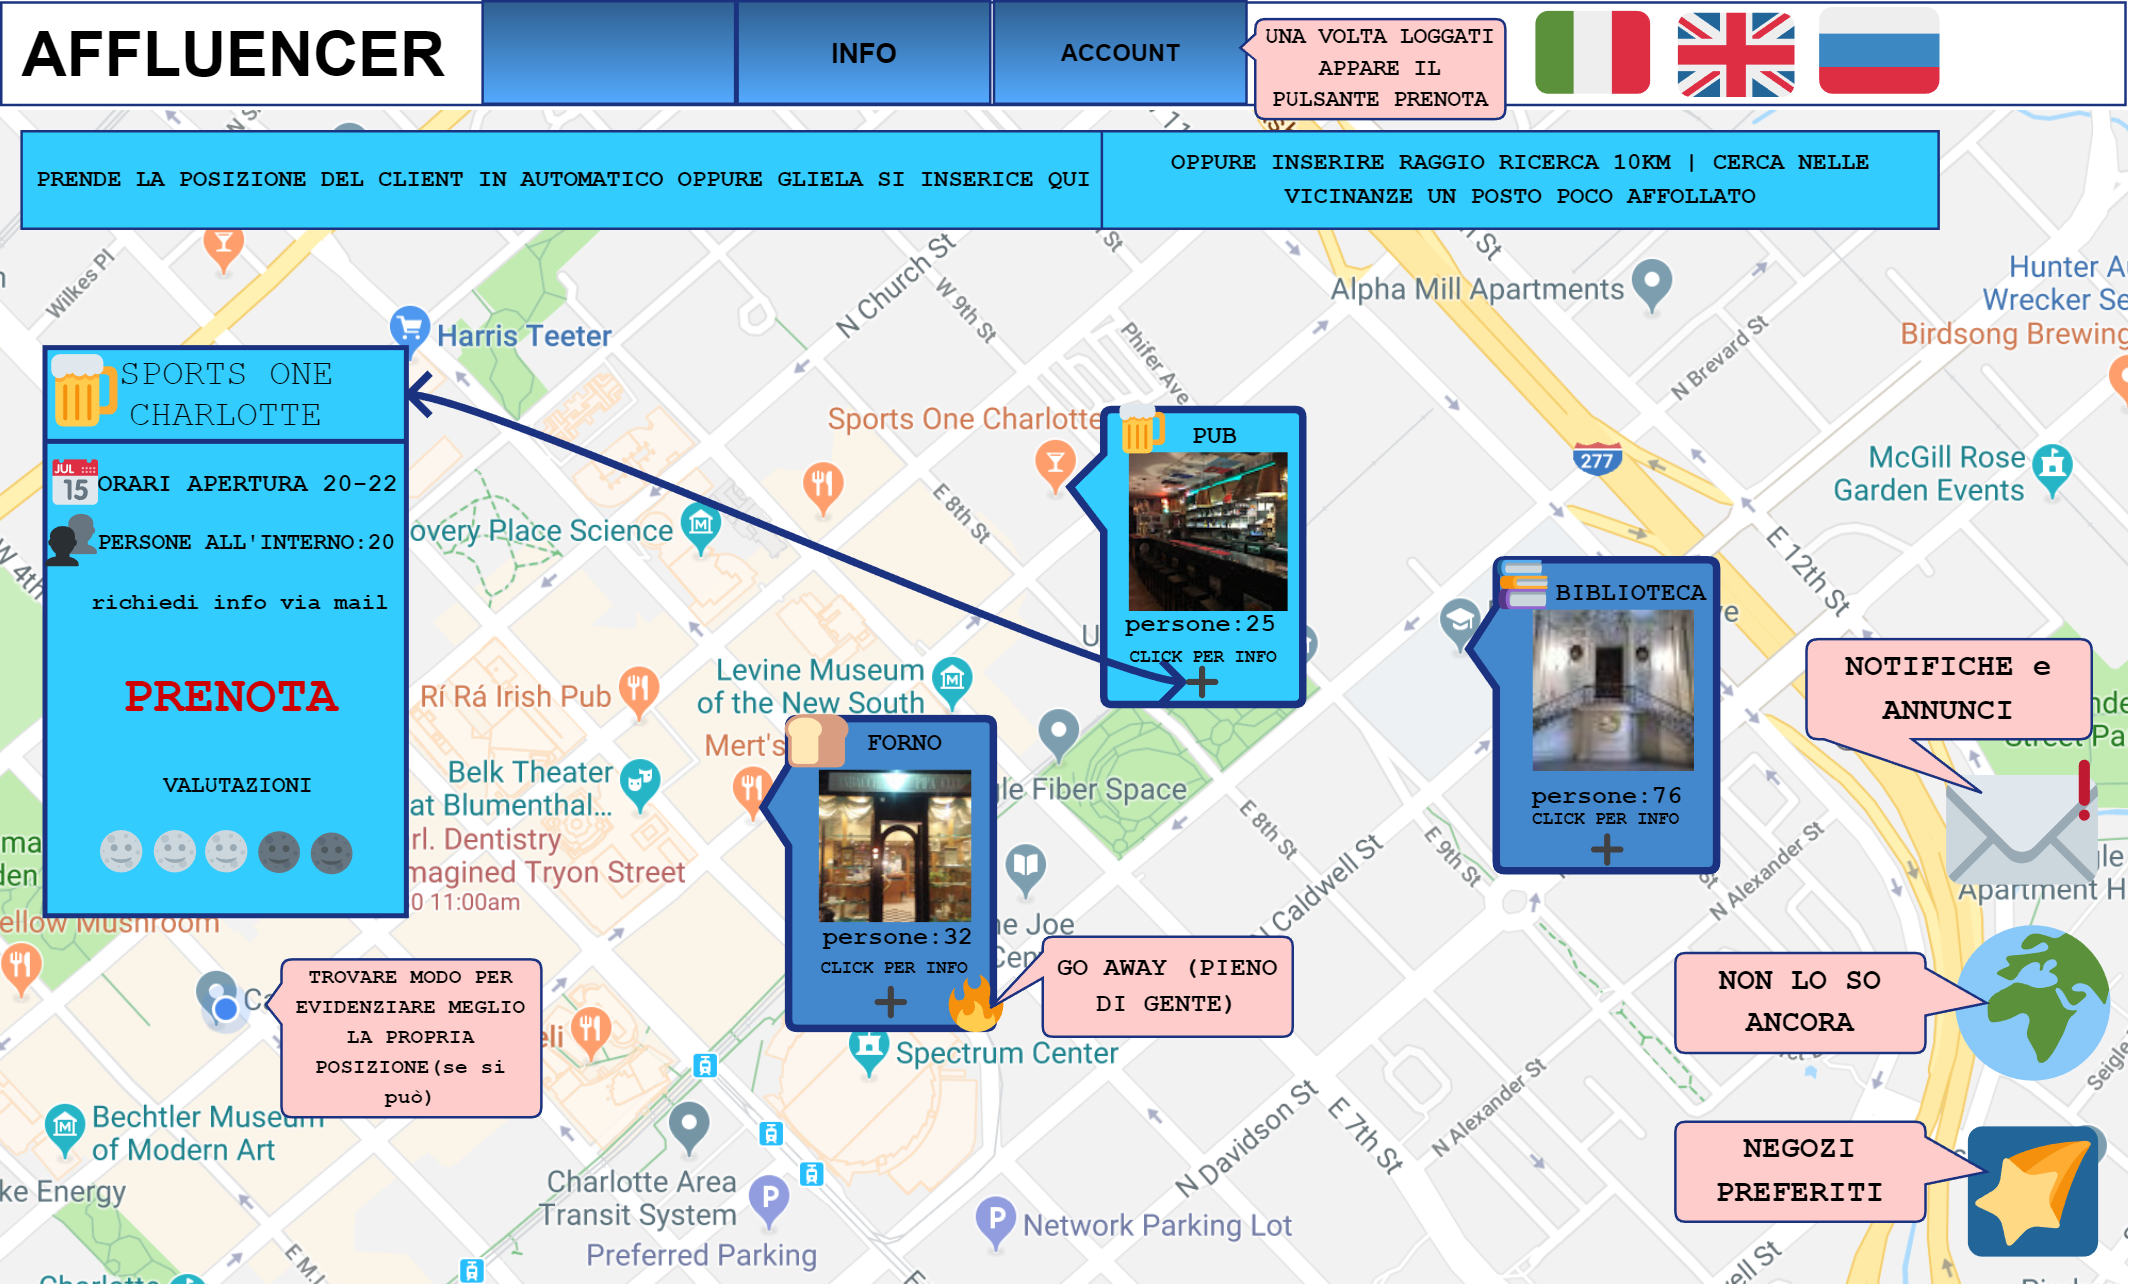
\includegraphics[width=\textwidth]{mockup_home.png}\\

Una barra di navigazione fissata in alto consente di accedere ai restanti servizi in qualsiasi momento.
%
Notifiche e negozi preferiti sono stati considerati elementi di elevata interazione, per cui sono presenti in basso a destra i rispettivi pulsanti.
%
Per gli utilizzatori del "dark theme" è possibile cambiare lo stile di visualizzazione dal pulsante posto in basso a sinistra.

Gli elementi della mappa sono icone corrispondenti alle attività registrati sul portale.
%
A ogni categoria di attività è associata la rispettiva icona.
%
Cliccando sulle icone dei negozi verrà visualizzata una scheda riassuntiva,che permette di visualizzare dei dati riassuntivi: indirizzo, orari, valutazione media (data dalle recensioni dei clienti), affluenza (in base agli ultimi dati registrati). Inoltre, è possibile effettuare una prenotazione direttamente dalla mappa, oppure visualizzare la pagina completa del negozio.
%
Visitando la pagina del negozio, se si utilizza un account cliente, è possibile lasciare una recensione. Un floating button permette di segnare il negozio come preferito.
%
Visitando la pagina con l’account appartenente al proprietario dell’attività, invece, è presente un form per la pubblicazione degli annunci, mentre il floating button permette di modificare la pagina, aggiornando i propri dati o rimuovendo gli annunci e i commenti alle recensioni. Annunci e recensioni sono strutturati per visualizzare solo la prima scheda, mentre le altre sono visualizzabili in un elenco collassabile, in modo analogo ai form di inserimento.
%

A seguire, nella pagina sono presenti i grafici che integrano i dati di sensori, segnalazioni e prenotazioni. In particolare, sono stati scelti due istogrammi e un grafico a linea. I due istogrammi indicano, rispettivamente: la media dell’affluenza oraria registrata dai sensori e segnalata dai clienti per il giorno corrente; una stima delle persone presenti nel negozio dall’ora successiva, basata sulle prenotazioni effettuate. Il grafico a linea mostra l’affluenza media allo stesso modo del primo istogramma, ma giornaliera e relativa alla settimana precedente.

\chapter{Tecnologie}

\textbf{Vue}: Utilizzando il framework Vue, è possibile gestire con facilità pagine web reattive, il che è fondamentale in un’applicazione come questa che dipende molto dalla reattività dei dati. Le pagine sono organizzate in termini di View, che includono Component al loro interno. Tra le view principali ci sono, ad esempio: Home, Profile, Store, Login, Register; tra i componenti principali invece si trovano: Navbar, LoginForm, StoreInfo, StoreReview, UserInfo, DayHistogram, ecc..

Le view si occupano principalmente di organizzare i componenti che le compongono all’interno del template, ed eventualmente di passare loro i \textit{prop} contenenti i dati di cui necessitano.
Infatti, la comunicazione dei dati in Vue è di tipo \textit{parent-to-child}: i dati scorrono dai componenti esterni verso quelli più interni, mentre una segnalazione nel verso opposto viene eseguita tramite la generazione di eventi. Ad esempio, i dati presenti in una view vengono passati ai componenti interni attraverso prop, e se i componenti necessitano di rispondere con altri dati, lo fanno generando un evento, in modo da non invertire il \textit{data flow}.

Nel caso dell’applicazione, i componenti che necessitano di richiedere dati al server per la loro inizializzazione lo fanno in fase di creazione (\textit{created() lifecycle hook}), in quanto risulta il più adatto per impostare il valore iniziale dei dati reattivi ed eventualmente passarli ai componenti figli, in quanto il DOM del componente non è ancora presente (il componente esiste ma non è ancora visualizzato) e di conseguenza viene introdotto meno ritardo. Al contrario, viene usato il (\textit{mounted() lifecycle hook}) nel caso ci sia bisogno di manipolare il DOM una volta che il componente è stato definitivamente inserito nella pagina.\\

\textbf{Vuetify}: Viene utilizzato il framework Vuetify in modo da avere a disposizione dei componenti pronti in stile \textit{material design}, nonchè diversi effetti grafici utili per creare un’applicazione dall’elevata usabilità.

Uno degli aspetti più utili e importanti di Vuetify è sicuramente il suo grid system, che permette di organizzare il template della pagina in righe e colonne, in modo simile a Bootstrap. Ogni riga e colonna può essere divisa in dodici parti, e vengono forniti diversi \textit{breakpoint} per permettere di costruire facilmente pagine web responsive. Inoltre, sono presenti diverse classi css preimpostate per facilitare lo styling delle pagine.\\

\textbf{Vue2Leaflet}: è una libreria basata su Leaflet per Vue che permette la creazione di mappe reattive. Ha una grande quantità di componenti personalizzabili ed è molto ben documentata. Tra i principali troviamo: 

\begin{itemize}

\item Tile-Layers: permette di caricare e visualizzare i riquadri che compongono la mappa, nel nostro caso ottenuti da OpenStreetMaps;
\item  Marker: un’icona personalizzabile che viene visualizzata nella mappa ad una certa latitudine/longitudine;
\item Popup: riquadro che si apre al click del Marker e permette di visualizzare informazioni aggiuntive;
\item Tooltip: per visualizzare informazioni sintetiche riguardanti il marker;
\end{itemize}

Questa libreria è stata fondamentale per la creazione della home del progetto, dove ad ogni negozio corrisponde un Marker e il Popup permette di visualizzare le informazioni principali.\\

\textbf{MongoDB}: database non-relazionale (NoSQL), perfettamente integrato con Node.js, che ha permesso una maggiore flessibilità delle strutture dati rispetto ad un database tradizionale. Nell’applicativo server viene usata la libreria Mongoose per interfacciarsi con maggiore facilità.


\chapter{Codice}
Di seguito sono elencate le principali parti di codice dei componenti.
\section{Home}
Per quanto riguarda la Home le parti di codice principali sono la geolocalizzazione del dispositivo utilizzato (se disponibile).

\begin{lstlisting}
    getUserPosition: async function() {
      // check if API is supported
      if (navigator.geolocation) {
        // get  geolocation
        navigator.geolocation.getCurrentPosition((pos) => {
          // set user location
          this.userLocation = latLng(pos.coords.latitude,     pos.coords.longitude);
        });
      }
    },
\end{lstlisting}

e la creazione dei marker con le informazioni e la categoria:

\begin{lstlisting}
for (var store of storeList.data) {
  for (var category of this.selectedCategories) {
    if (category == store.category) {
      this.markers.push({
        id: store._id,
        text: store.name,
        value: latLng(store.location.coordinates),
        category: store.category,
      });
    }
  }
}
\end{lstlisting}
\pagebreak
\section{Profile}

Per quanto riguarda il profilo del cliente vengono visualizzati oltre ai dati personali anche i negozi preferiti, le prenotazioni effettuate e le reviews

\begin{lstlisting}
<v-card elevation="5">
  <v-btn fab fixed top right @click="$store.commit('toggleSettings')" color="primary" class="mt-16">
    <v-icon>mdi-cog</v-icon>
  </v-btn>
  <userInfo :userData="userData"/>
  <userFavoriteStores/>
  <userReservations/>
  <userReviews/>
</v-card>
\end{lstlisting}

\section{Store}
Nella pagina del negozio vengono visualizzate le informazioni riguardanti gli annunci, le reviews, le prenotazioni dei clienti e i grafici sull’affluenza.

\begin{lstlisting}
<v-row v-if="!$store.state.config.settings" justify="center">
  <v-col cols="10" class="mt-5">
    <span class="text-h4">{{ storeData.name }}</span>
  </v-col>
</v-row>
                
<v-row justify="center">
  <v-col cols="10" md="4">
    <storeInfo :storeData="storeData"/>
  </v-col>
  <v-col cols="10" md="8">
    <storeAnnouncements/>
    <storeReviews/>
    <userReservations v-if="isStore && isOwner" />
  </v-col>
</v-row>
<v-row justify="center">
  <v-col cols="10">
    <storeStats/>
  </v-col>
</v-row>
\end{lstlisting}



\chapter{Test}

Il metodo di testing ha incluso diversi strumenti. Alcuni hanno coperto solo lo sviluppo back-end, solo il front-end oppure entrambi.\\

\textbf{User story}: la base di partenza per la validazione del progetto, da cui sono state generati anche i requisiti. Ogni user story creata rappresenta una specifica funzione o un insieme di esse, in modo tale che fossero coperto l’intero sistema.
L’uso della piattaforma da parte di componenti esterni al team ha permesso di osservare l’usabilità del sistema e dell’efficienza delle funzioni. Facendo usare il loro device preferito abbiamo osservato come l’utente abbia reagito all’interfaccia e seguito la sua user experience.\\

\textbf{Piattaforma Insomnia}: per testare la comunicazione con il server di backend è stato utilizzato il software Insomnia, lo stesso usato per sviluppare le API. Sono state create variabili di ambiente specifiche per simulare una particolare istanza della piattaforma, velocizzando il processo.\\

\textbf{In-browser debugging}: grazie agli strumenti per sviluppatori già integrati nel browser eventuali errori sono stati velocemente gestiti. Le variabili di debug inoltre facilitano il passo-a-passo del codice per scovare i casi di funzionamento errato.


\chapter{Deployment}

Il progetto si compone di due software indipendenti, ovvero il server e l’applicazione Vue.

\begin{itemize}
\item Entrambe vengono avviate mediante linea di comando, assicurandosi che prima di avviare il server è necessario far partire il servizio di MongoDB sulla porta di default.
\item Entrambe sono sviluppate e fatte funzionare su tecnologia Node.js, per cui al momento dell’installazione viene utilizzata l’utility npm per scaricare le librerie necessarie al funzionamento.
\item Sebbene l’applicazione Vue sia indipendente a livello di installazione non è in grado di operare correttamente senza che sia stato precedentemente avviato il server.
\item I due processi possono operare sulla stessa macchina di installazione, poiché le porte utilizzate sono diverse tra di loro.
\end{itemize}

Una volta copiati i sorgenti nella/e macchina/e designata/e si procede nei seguenti modi:

\begin{itemize}
\item \textbf{Server}: avviare il servizio di MongoDB ed eseguire il comando \texttt{mongorestore} per caricare il contenuto della cartella \texttt{resources/demo}. Installare quindi le librerie mediante il comando \texttt{npm install}, infine avviare il processo mediante \texttt{npm start}.
Per riempire il database con alcuni dati simulati, utilizzare il comando \texttt{npm run fill}. Questo comando avvierà la funzione contenuta nel file \texttt{server/filler.js}, dove è possibile modificare la data di inizio e fine simulazione.
\item \textbf{Applicazione Vue}: installare le librerie mediante il comando \texttt{npm install}, dopodiché avviare il processo mediante \texttt{npm run serve}.
\end{itemize}

A questo punto è possibile collegarsi all’applicazione utilizzando l’indirizzo IP della macchina e la porta 8080.

\chapter{Conclusioni}

La versione finale del progetto è risultata coerente con ciò che era stato progettato in fase di mockup, grazie anche all’utilizzo della metodologia Kanban tramite il software Trello, che ci ha permesso di essere molto flessibili nello sviluppo. Inoltre, la creazione di mockup per le pagine e la definizione di user stories è stata fondamentale per impostare una prima organizzazione del lavoro.

Il framework Vue è risultato essere il più adatto e intuitivo per la gestione di questo tipo di applicazione, avendo a che fare con pagine web che devono interagire con diversi dati allo stesso tempo in modo reattivo.

Inoltre, l’utilizzo di librerie e framework aggiuntivi come Vuetify, Leaflet e Axios ci ha fornito molti spunti su come affrontare lo sviluppo di applicazioni di questo tipo.

Per quanto riguarda l’applicazione, si è potuto verificare nelle fasi di testing, grazie anche al feedback ricevuto, l’elevata usabilità data dall’interfaccia reattiva. Inoltre, l’aggregazione di dati provenienti da sensori IoT e da utenti, uniti alla \textit{data visualization}, la rendono lo strumento ideale per risolvere questo problema, che al giorno d’oggi è diventato fin troppo comune.
\end{document}
